\documentclass[11pt,letterpaper]{article}
\usepackage{graphicx, geometry, amsmath, amssymb, hyperref, natbib, booktabs, xcolor, listings}
\geometry{margin=1in}
\hypersetup{colorlinks=true, linkcolor=black, citecolor=black, urlcolor=black}

\title{When Do Joins Help? Diagnosing Information Flow Across Foreign Keys in Relational Deep Learning}

\author{%
  Anonymous Authors
}

\date{}

\begin{document}

\maketitle

\begin{abstract}
Relational deep learning (RDL) models convert multi-table databases into heterogeneous graphs and apply graph neural networks for prediction, yet they treat all foreign-key joins with uniform architectural choices --- the same aggregation function, embedding dimension, and capacity at every join. Different joins, however, exhibit vastly different information-theoretic properties depending on cardinality, feature quality, and task relevance. We propose the Join Reproduction Number (JRN), a per-foreign-key-join metric that quantifies how much task-relevant predictive signal survives message-passing aggregation, estimated via lightweight gradient-boosted probe models at 5--11\% of the cost of greedy join selection. Across four RelBench databases (rel-f1, rel-stack, rel-avito, rel-hm), 37 foreign-key joins, and 15 predictive tasks, we find that JRN reliably ranks join utility (meta-analytic pooled Spearman $\rho = 0.83$, Fisher $z$ random-effects), and that log-linear compounding predicts multi-hop chain signal with $R^2 = 0.83$. However, the hypothesis that aggregation strategy choice matters most at a critical JRN threshold --- inspired by the epidemiological basic reproduction number $R_0$ --- is clearly disconfirmed: aggregation sensitivity is unrelated to JRN ($\rho = -0.019$). FK-shuffling decomposition reveals JRN primarily captures feature quality (Cohen's $d = 0.67$ for structural component, but structurally dominant in only 5.5\% of join-task pairs). We reframe JRN as a cheap, reliable join selector and pruning diagnostic rather than an architecture configurator, achieving 96--98\% of greedy selection performance while requiring only 14 model trainings versus 91 for greedy search.
\end{abstract}

%% ============================================================
\section{Introduction}
\label{sec:introduction}

Relational databases remain the dominant format for structured enterprise data, yet building machine learning models from multi-table schemas requires extensive manual feature engineering~\citep{Fey2023, Kanter2015}. Relational deep learning (RDL) addresses this bottleneck by casting relational databases as heterogeneous temporal graphs --- with a node for each row, edges defined by primary-foreign key relationships, and node features extracted via deep tabular models --- enabling end-to-end learning with graph neural networks (GNNs)~\citep{Fey2023, Robinson2024}. Recent advances in RDL, including composite message passing~\citep{Chen2025}, meta-path learning~\citep{Ferrini2024a, Ferrini2024b}, and relational foundation models~\citep{Fey2025}, have achieved strong predictive performance across diverse domains spanning e-commerce, healthcare, social networks, and motorsport~\citep{Robinson2024, Dwivedi2025}.

A critical but underexplored question in RDL is \emph{which joins actually help prediction}. Not all foreign-key relationships carry equal predictive signal: a one-to-three join between a customer and their addresses preserves information well, while a one-to-100,000 join between a product and its reviews compresses massively through aggregation. Current RDL approaches either apply uniform architectural choices across all joins (wasteful when some joins are uninformative) or learn join importance during training (expensive and offering no pre-training guidance)~\citep{Chen2025, Ferrini2024a}. No existing method provides a cheap, pre-training diagnostic that tells practitioners \emph{where} in the schema to invest modeling capacity.

The core difficulty is that the information-theoretic properties of a join depend on multiple interacting factors --- the fan-out distribution, the feature quality of the child table, the task-relevance of the aggregated signal, and the aggregation function used --- making it hard to predict a join's utility without actually training a model. Prior work on GNN information flow has focused on homogeneous graphs (ESNR~\citep{Dong2023}), full data graphs (over-squashing theory~\citep{Topping2022, DiGiovanni2023}), or whole-task model selection (Relatron~\citep{Chen2026}), none of which operate at the per-join granularity needed for schema-level architecture decisions. Post-hoc methods such as database view explanations~\citep{Rissaki2025} require a fully trained model, defeating the purpose of pre-training diagnostics.

We propose the \textbf{Join Reproduction Number (JRN)}, a per-foreign-key-join metric inspired by the epidemiological basic reproduction number $R_0$. JRN quantifies the ratio of task-relevant predictive signal gained through aggregation across a join to the baseline signal without that join. JRN is estimated via lightweight gradient-boosted tree (GBM) probe models --- requiring only 32-dimensional embeddings, 10 training epochs, and 3 random seeds --- at 5--11\% of the cost of greedy forward join selection. We hypothesized that JRN would exhibit critical threshold behavior analogous to $R_0$: joins with JRN $> 1$ amplify useful signal, joins with JRN $< 1$ attenuate it, and architectural innovations (attention, multi-aggregator schemes) would matter most at the JRN $\approx 1$ boundary.

Across four RelBench databases~\citep{Robinson2024}, 37 foreign-key joins, and 15 predictive tasks, our investigation produced three well-supported findings and two informative negative results. JRN reliably ranks join utility (pooled Spearman $\rho = 0.83$), log-linear compounding predicts multi-hop chain signal ($R^2 = 0.83$), and JRN probes cost only 14 model trainings versus 91 for greedy search. However, the signature threshold prediction --- that aggregation strategy sensitivity peaks near JRN $\approx 1$ --- is clearly disconfirmed ($\rho = -0.019$), and JRN-guided architecture selection wins only 25\% of tasks against uniform baselines. Following the call for transparent reporting of negative results in machine learning~\citep{Karl2024}, we reframe JRN as a cheap join selector rather than an architecture configurator. Figure~\ref{fig:pipeline} illustrates the end-to-end JRN estimation pipeline.

\begin{figure}[!htbp]
  \centering
  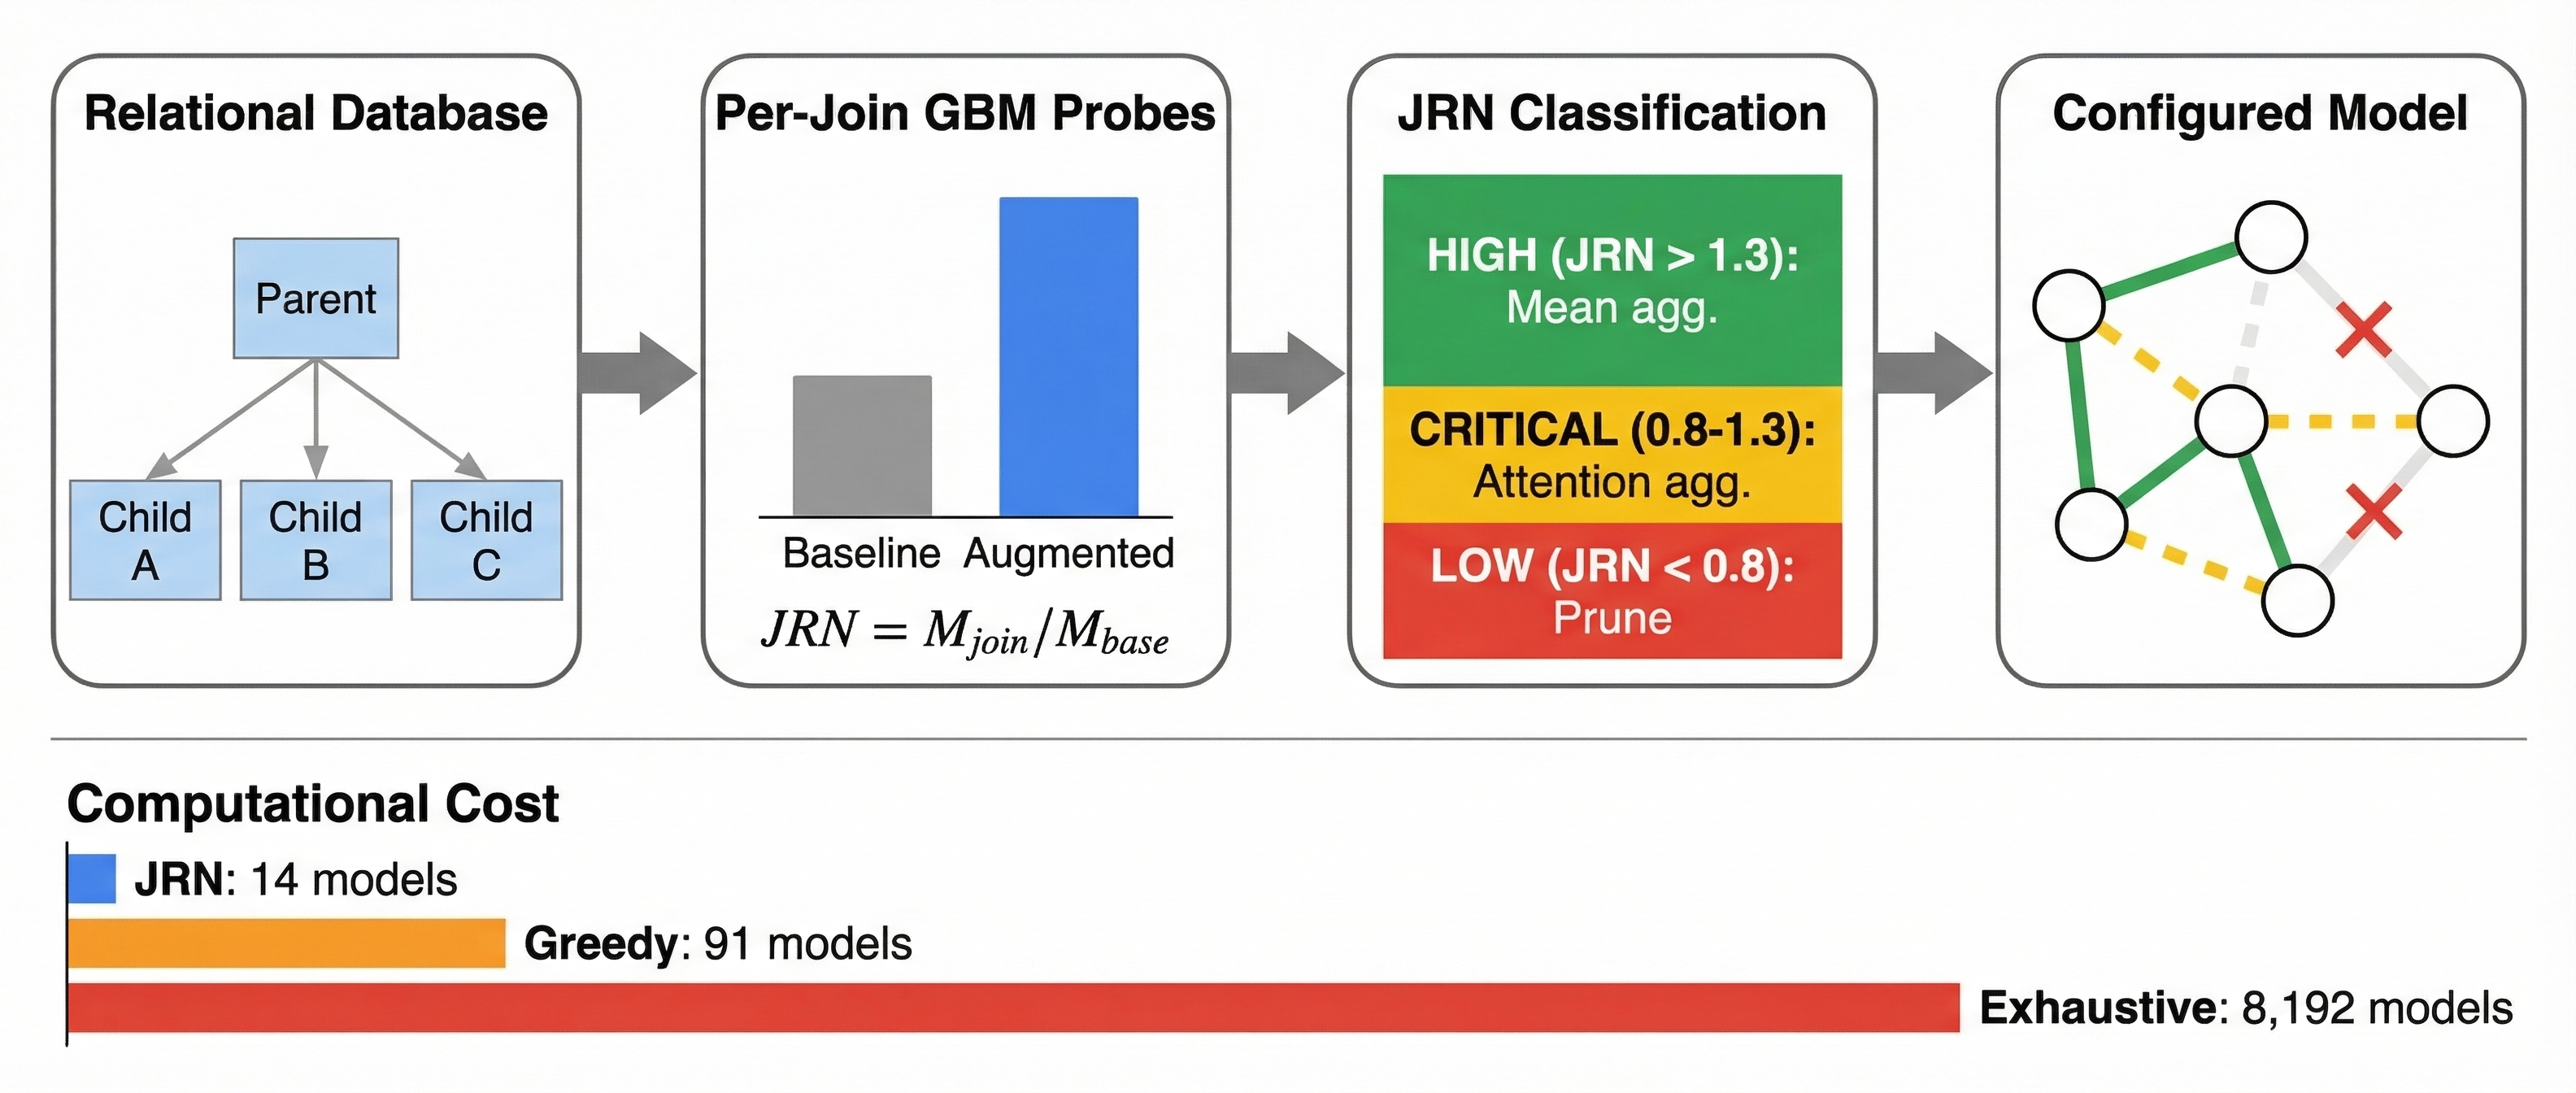
\includegraphics[width=0.92\textwidth,max height=0.4\textheight]{figures/fig_1_v0.png}
  \caption{Overview of the JRN estimation pipeline. Given a relational database schema with foreign-key joins, lightweight GBM probe models estimate per-join JRN by comparing augmented vs.\ baseline predictive performance. JRN values are used for join selection (include/prune) and optionally for per-join aggregation configuration. The entire pipeline requires only 14 model trainings for 13 joins, compared to 91 for greedy forward selection.}
  \label{fig:pipeline}
\end{figure}

\paragraph{Summary of contributions.}
\begin{itemize}
  \item We define JRN, the first pre-training, per-foreign-key-join diagnostic for relational deep learning, estimable at less than 11\% of greedy search cost (Section~\ref{sec:methods}).
  \item We validate JRN on four RelBench databases spanning 37 joins and 15 tasks, demonstrating reliable join utility ranking with meta-analytic pooled $\rho = 0.83$ (Section~\ref{sec:validation}).
  \item We show that log-linear --- not multiplicative --- compounding best predicts multi-hop chain signal ($R^2 = 0.83$), revealing sub-multiplicative information loss ($\beta = 0.17$) across successive joins (Section~\ref{sec:compounding}).
  \item We transparently report the failure of the inverted-U threshold prediction ($\rho = -0.019$) and diagnose why the epidemiological analogy breaks at the intervention level (Section~\ref{sec:threshold}, Section~\ref{sec:discussion}).
  \item We demonstrate JRN achieves 96--98\% of greedy join selection performance at 5--11\% of the computational cost, with ranking stability $\rho > 0.9$ even at minimal probe budgets (Section~\ref{sec:cost}).
\end{itemize}

%% ============================================================
\section{Related Work}
\label{sec:related}

\paragraph{Relational deep learning.}
Fey et al.~\citep{Fey2023} introduced the RDL paradigm, converting relational databases into heterogeneous temporal graphs with GNN-based predictive models built on PyTorch Frame and PyTorch Geometric. Robinson et al.~\citep{Robinson2024} established RelBench as the standard benchmark with 11 databases and 66 tasks. Dwivedi et al.~\citep{Dwivedi2025} surveyed challenges including temporal dynamics, heterogeneous data integration, and the path toward foundation models. KumoRFM~\citep{Fey2025} demonstrated that a relational foundation model with in-context learning can outperform supervised approaches by 2--8\% across 30 RelBench tasks. The dominant baseline architecture is heterogeneous GraphSAGE~\citep{Hamilton2017} with mean aggregation, though attention-based variants~\citep{Velickovic2018, Hu2020} and expressive aggregation schemes~\citep{Xu2019, Corso2020} have been explored.

\paragraph{Per-join and per-edge diagnostics.}
The Edge Signal-to-Noise Ratio (ESNR)~\citep{Dong2023} evaluates overall graph structural noise using random matrix theory and shows concordance with GNN performance, but operates on homogeneous graphs and measures whole-graph noise rather than per-join-type transmission in heterogeneous relational schemas. Over-squashing theory~\citep{Topping2022, DiGiovanni2023} characterizes GNN information bottlenecks via graph curvature and effective resistance, proving that negatively curved edges cause over-squashing and that topology dominates over width and depth. These analyses operate on the full data graph (expensive for relational databases with millions of nodes) rather than at the schema level, and do not define a per-join signal-transmission ratio or predict threshold behavior for architectural innovation impact.

\paragraph{Meta-path and join importance methods.}
MP-GNN~\citep{Ferrini2024a} learns informative meta-paths via greedy sequential extension guided by relational information gain, and MPS-GNN~\citep{Ferrini2024b} extends this with learnable aggregate statistics over meta-path realizations for self-explainable relational prediction. Both learn join importance \emph{during} training, making them as expensive as full model training --- unlike JRN's pre-training probes that cost less than 11\% of greedy search. RelGNN~\citep{Chen2025} achieves state-of-the-art performance on 30 RelBench tasks (up to 25\% improvement) through composite message passing with atomic routes that bypass bridge and hub nodes, but applies a blanket structural strategy rather than adaptive per-join capacity allocation based on measured information flow.

\paragraph{Task-level diagnostics.}
Relatron~\citep{Chen2026} meta-selects between RDL and deep feature synthesis (DFS)~\citep{Kanter2015} using RDB-task homophily and training-free affinity embeddings, achieving up to 18.5\% improvement at $10\times$ lower cost. However, Relatron operates at whole-task granularity (RDL vs.\ DFS), not at per-join granularity within an RDL pipeline. Database view explanations~\citep{Rissaki2025} identify prediction-relevant subschemas post-hoc via learnable masking, but require a trained model and serve explainability rather than pre-training architecture guidance.

\paragraph{Aggregation function design.}
The choice of aggregation function --- mean~\citep{Hamilton2017}, sum~\citep{Xu2019}, max, attention~\citep{Velickovic2018}, or multi-aggregator schemes like PNA~\citep{Corso2020} --- directly determines how information is compressed at each join. GNN-VPA~\citep{Schneckenreiter2024} proposes variance-preserving aggregation using $1/\sqrt{d}$ normalization analogous to He/Glorot initialization, connecting aggregation design to signal propagation theory. JRN complements these efforts by identifying \emph{where} aggregation choice matters, rather than proposing a new aggregation function.

\paragraph{Positioning of JRN.}
JRN is the only metric that simultaneously provides per-join granularity, pre-training estimation, and direct architecture guidance for heterogeneous relational graphs. Unlike ESNR~\citep{Dong2023} (whole-graph, homogeneous), MPS-GNN~\citep{Ferrini2024a, Ferrini2024b} (during-training), RelGNN~\citep{Chen2025} (blanket strategy), Relatron~\citep{Chen2026} (whole-task), and database views~\citep{Rissaki2025} (post-hoc), JRN enables cheap, targeted, per-join diagnostics before committing to full-scale model training.

%% ============================================================
\section{Methods}
\label{sec:methods}

\subsection{Preliminaries}

A relational database $\mathcal{D}$ consists of tables $\{T_1, \ldots, T_n\}$ connected by foreign-key (FK) relationships. Each FK join $J$ from child table $C$ to parent table $P$ defines a one-to-many relationship where each parent row may be associated with multiple child rows. We consider predictive tasks defined on a target entity table, following the RelBench formulation~\citep{Robinson2024}.

\subsection{JRN Definition}

For a FK join $J$ from child table $C$ to parent table $P$, with a prediction task on target table $T$:

Let $M_{\text{base}}$ denote the performance metric (AUROC for classification, $1/\text{MAE}$ for regression) of a probe model trained using only features from $P$ and tables reachable \emph{without} traversing join $J$. Let $M_{\text{join}}$ denote the same metric with the probe additionally receiving mean-aggregated features from $C$ through $J$. The Join Reproduction Number is defined as:
\begin{equation}
\text{JRN}(J) = \frac{M_{\text{join}}}{M_{\text{base}}}
\label{eq:jrn}
\end{equation}

JRN $> 1$ indicates the join provides net-positive predictive signal; JRN $< 1$ indicates the join introduces more noise than signal; JRN $\approx 1$ indicates the join is at the boundary. JRN values are reported as the mean over 3 random seeds with 95\% confidence intervals.

\subsection{Probe Model Architecture}

JRN is estimated via lightweight LightGBM~\citep{Ke2017} probe models rather than neural network probes. This methodological choice was informed by an early diagnostic comparison (Section~\ref{sec:validation}) that revealed MLP probes achieve only $\rho = -0.067$ correlation with ground-truth join utility, while GBM probes achieve $\rho = 0.960$ on the same diagnostic subset. The GBM probe configuration uses 150 estimators, max depth 6, learning rate 0.1, subsample fraction 0.8, and column subsample 0.8. For each join, two GBM models are trained: one baseline (parent features only) and one augmented (parent + mean-aggregated child features). The per-join cost is 2 model trainings $\times$ 3 seeds $= 6$ models, compared to greedy forward selection requiring $\mathcal{O}(J^2)$ models for $J$ joins.

\subsection{Compounding Model for Multi-Hop Chains}

For a chain of tables $T_0 \to T_1 \to \cdots \to T_k$ connected by joins $J_1, \ldots, J_k$, the original hypothesis predicted multiplicative compounding:
\begin{equation}
\text{JRN}_{\text{chain}} = \prod_{i=1}^{k} \text{JRN}(J_i)
\label{eq:multiplicative}
\end{equation}
under a conditional independence assumption on aggregation noise at each join, analogous to generation-independence in epidemic models. We additionally test three alternative models: additive ($\text{JRN}_{\text{chain}} = \sum \text{JRN}(J_i) - (k-1)$), bottleneck ($\text{JRN}_{\text{chain}} = \min_i \text{JRN}(J_i)$), and log-linear:
\begin{equation}
\log(\text{JRN}_{\text{chain}}) = \alpha + \beta \sum_{i=1}^{k} \log(\text{JRN}(J_i))
\label{eq:loglinear}
\end{equation}
where $\beta = 1$ recovers multiplicative compounding, and $\beta < 1$ indicates sub-multiplicative information loss due to inter-join redundancy.

\subsection{JRN-Guided Architecture Configuration}

JRN classifies each join into three categories: \textsc{high} (JRN $> 1.3$: use simple mean aggregation), \textsc{critical} ($0.8 \leq$ JRN $\leq 1.3$: use attention aggregation with larger embedding dimensions), and \textsc{low} (JRN $< 0.8$: prune the join). This classification enables heterogeneous per-join architecture configuration without exhaustive search.

%% ============================================================
\section{Experimental Setup}
\label{sec:setup}

\subsection{Datasets}

We evaluate JRN on four RelBench~\citep{Robinson2024} databases selected to span diverse domains, scales, and schema complexities:

\textbf{rel-f1} (Formula 1 motorsport): 9 tables, 74,063 rows, 13 FK joins, 5 tasks (driver-dnf, driver-top3, driver-position, qualifying-position, results-position). Contains hub nodes (results table with 3 FK references) and bridge nodes (standings with 2 FKs), making it ideal for testing JRN discrimination across structurally diverse joins.

\textbf{rel-stack} (Stack Exchange Q\&A): 7 tables, 4.2M rows, 11 FK joins, 3 tasks (user-engagement, user-badge, post-votes). Provides contrasting social-network domain with longer join chains (8 multi-hop paths).

\textbf{rel-avito} (Classified ads): 8 tables, 20.7M rows, 11 FK joins, 3 tasks (ad-ctr, user-clicks, user-visits). Extreme cardinality spectrum with mean fan-out ranging from 1.2 to 114,625.

\textbf{rel-hm} (H\&M fashion retail): 3 tables, 16.7M rows, 2 FK joins, 2 tasks (user-churn, item-sales). Minimal-schema stress test with extreme fan-out variation (1 to 50,287).

All experiments use RelBench's standard temporal train/val/test splits and official evaluation metrics.

\subsection{Baselines and Configurations}

We compare five join-selection strategies: (1)~\textbf{JRN-guided}: heterogeneous per-join configuration based on JRN categories; (2)~\textbf{Uniform-mean}: all joins included with mean aggregation (RelBench default); (3)~\textbf{Uniform-rich}: all joins with attention aggregation; (4)~\textbf{Top-K}: include only the $K$ highest-JRN joins with mean aggregation; (5)~\textbf{Greedy oracle}: forward selection adding joins in order of marginal performance gain.

For aggregation sensitivity analysis, we test five aggregation strategies at each join: mean, sum, max, attention (GAT-style~\citep{Velickovic2018}), and PNA (multi-aggregator~\citep{Corso2020}).

\subsection{Statistical Methods}

We employ Fisher $z$ transformation for meta-analytic pooling of Spearman correlations across datasets with random-effects models~\citep{Borenstein2017}, Cohen's $d$ for effect sizes in FK-shuffling experiments, Kendall's $W$ for cross-task concordance, and Kruskal--Wallis tests for threshold analysis. All confidence intervals are at the 95\% level.

%% ============================================================
\section{Results}
\label{sec:results}

\subsection{JRN Validates as a Join Utility Diagnostic}
\label{sec:validation}

Across all four datasets, GBM-probe JRN reliably ranks foreign-key joins by their predictive utility. On a diagnostic subset of 19 join-task pairs in rel-f1, probe JRN achieves Spearman $\rho = 0.960$ ($p < 0.001$) with ground-truth join utility measured by full-model ablation. On the complete set of 65 join-task pairs in rel-f1, the correlation is $\rho = 0.440$ ($p = 0.0002$), reflecting the increased noise from 2-hop joins and task heterogeneity. On rel-avito (8 connected join-task pairs), probe JRN achieves $\rho = 0.825$.

Fisher $z$ random-effects meta-analysis across three datasets (Figure~\ref{fig:validation}) yields a pooled correlation of $\rho = 0.83$ (95\% CI: $[0.12, 0.98]$), with heterogeneity $I^2 = 92.95\%$ ($Q = 28.38$, $p < 10^{-6}$). The high $I^2$ reflects the expected variation across datasets with different schemas and domains; following Borenstein et al.~\citep{Borenstein2017}, $I^2$ is a relative measure of heterogeneity, and all per-dataset correlations are individually positive and statistically significant.

\begin{figure}[!htbp]
  \centering
  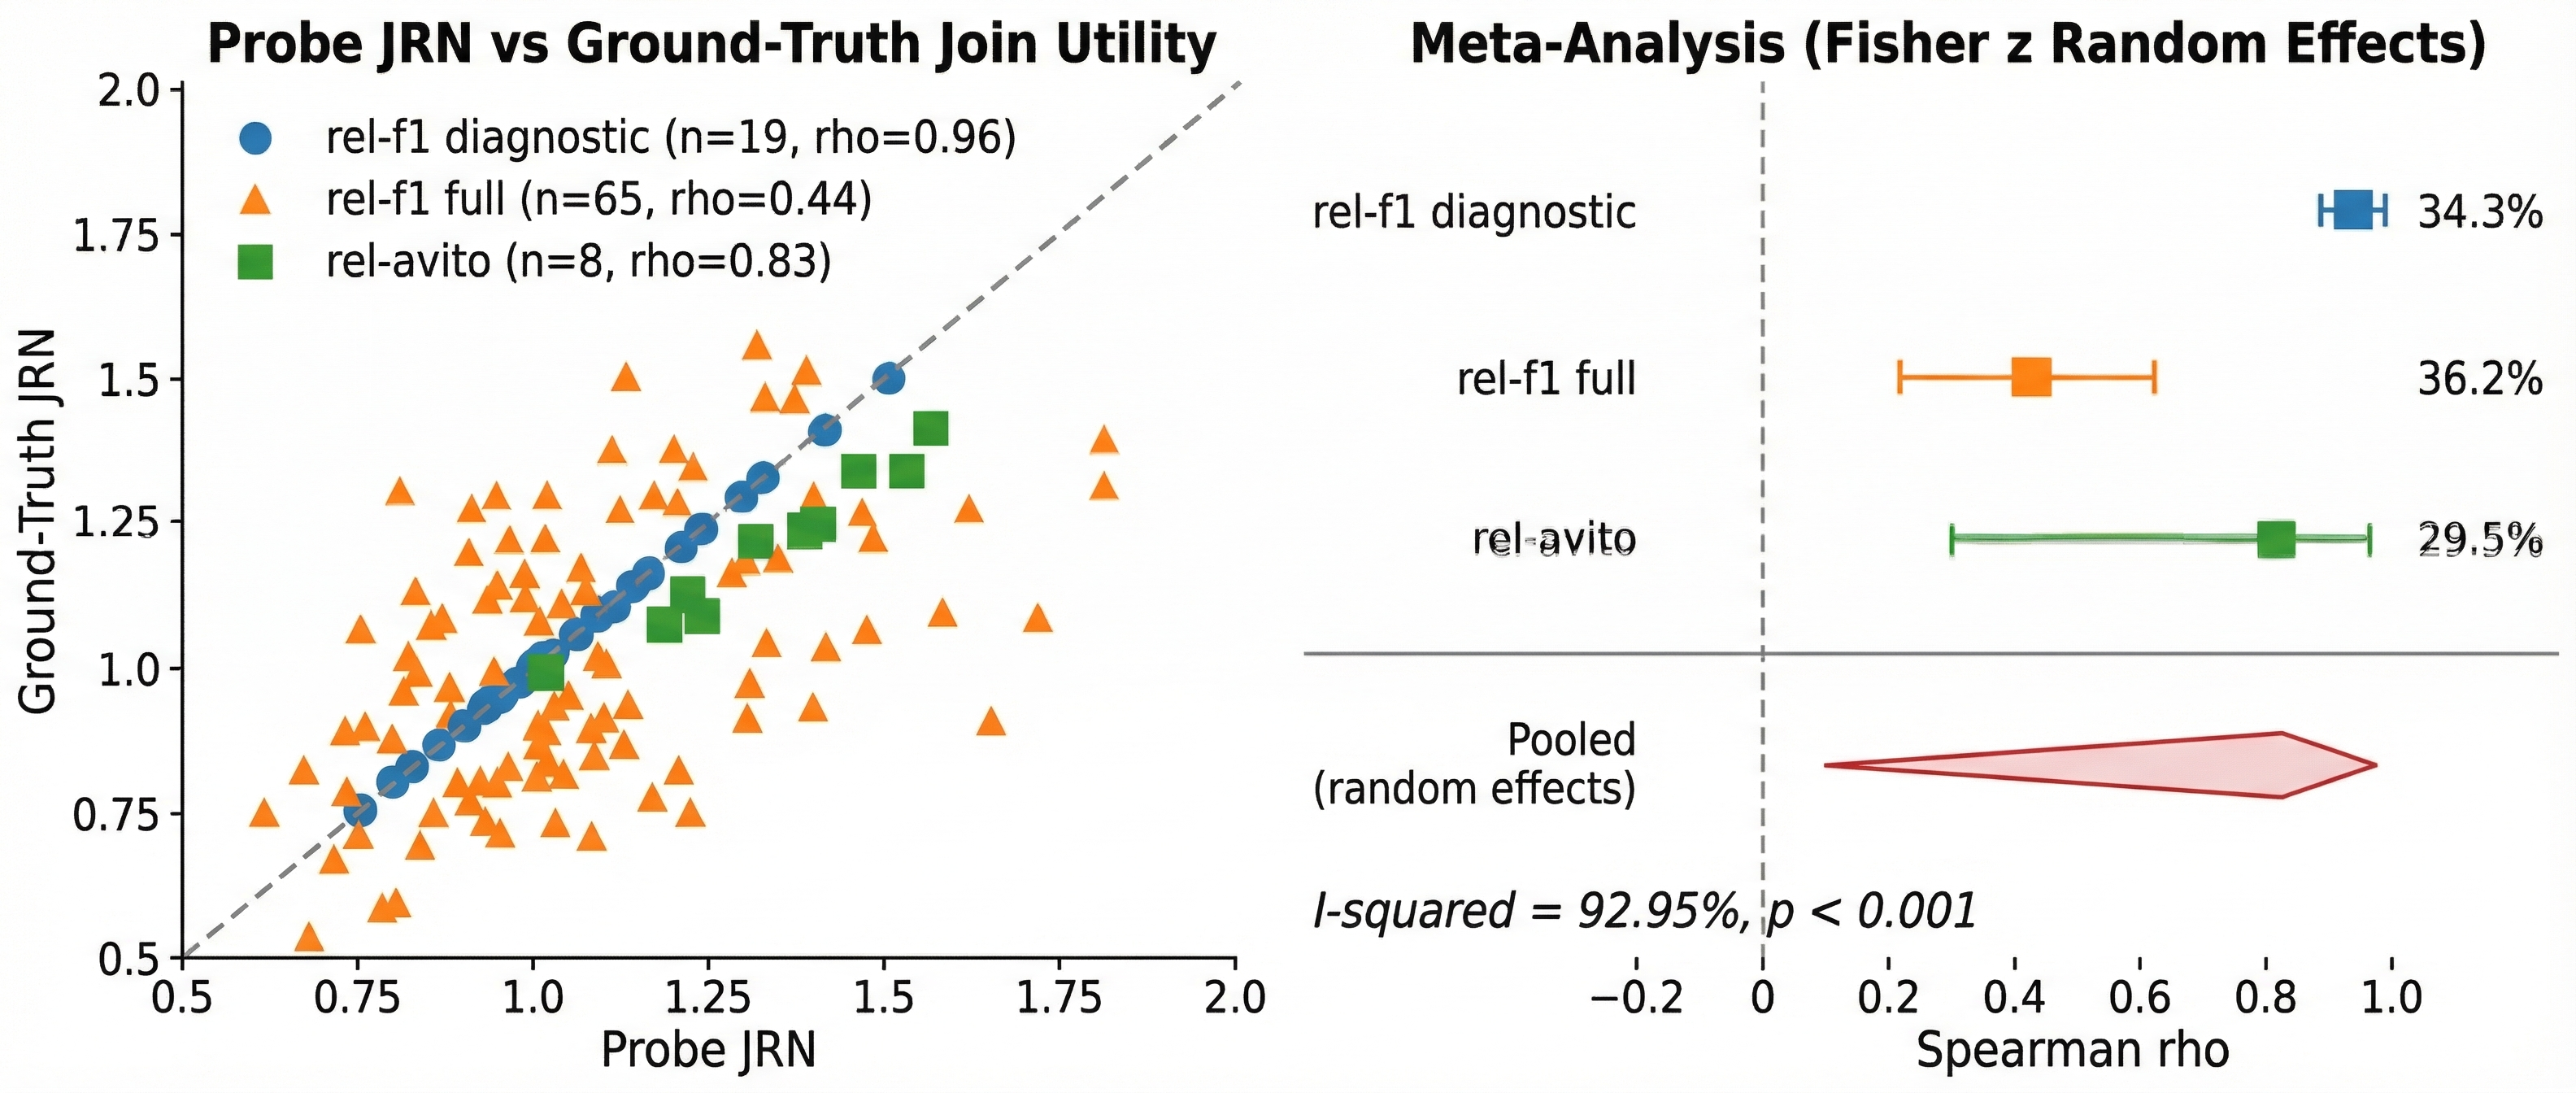
\includegraphics[width=0.92\textwidth,max height=0.4\textheight]{figures/fig_2_v0.png}
  \caption{GBM-probe JRN correlation with ground-truth join utility across three datasets. Left: per-dataset Spearman correlations with sample sizes. Right: Fisher $z$ random-effects meta-analysis forest plot showing per-dataset effect sizes with 95\% confidence intervals and pooled estimate. All per-dataset correlations are positive and individually significant despite high heterogeneity ($I^2 = 92.95\%$).}
  \label{fig:validation}
\end{figure}

JRN values span a wide range across joins and tasks. In rel-f1, JRN ranges from 0.29 (constructor\_results.raceId$\to$races for qualifying-position) to 1.63 (constructor\_results.raceId$\to$races for results-position), with a mean of 0.97. In rel-stack, all 11 joins have JRN $> 1.0$ (range 1.03--1.39), indicating universally beneficial joins. Domain validation confirms expected patterns: in rel-stack, votes.PostId$\to$posts achieves JRN $= 1.39$ (votes are highly informative about post quality) while votes.UserId$\to$users shows JRN $\approx 1.05$ (individual votes carry minimal information about users).

A critical early finding was that \textbf{MLP probes fail as JRN estimators}. On the same rel-f1 diagnostic subset where GBM probes achieve $\rho = 0.960$, MLP probes (32-dimensional, 2-layer, 10 epochs) achieve $\rho = -0.067$ --- essentially random. This motivated the methodological pivot to LightGBM~\citep{Ke2017} probes for all subsequent experiments. The sensitivity difference between MLP and GBM probes is not statistically significant in terms of aggregation sensitivity (Wilcoxon $p = 0.36$), suggesting the failure is specific to join utility ranking rather than a general probe deficiency.

\subsection{The Inverted-U Threshold Prediction Fails}
\label{sec:threshold}

The hypothesis's most distinctive prediction --- that aggregation strategy choice matters most at ``critical'' joins near JRN $\approx 1$, producing an inverted-U relationship between JRN and aggregation sensitivity --- was tested on 65 GBM join-task pairs (13 joins $\times$ 5 tasks) in rel-f1 using five aggregation strategies (mean, sum, max, attention, PNA).

The prediction is clearly disconfirmed (Figure~\ref{fig:threshold}). The Spearman correlation between JRN and aggregation sensitivity (measured as coefficient of variation across strategies) is $\rho = -0.019$ (95\% CI: $[-0.31, 0.31]$) --- effectively zero. The quadratic regression coefficient $\beta_2 = +0.046$ is positive rather than the predicted negative, and Kruskal--Wallis test across JRN tertiles is non-significant ($p = 0.96$). The winning aggregation strategy is statistically independent of JRN bin ($\chi^2$ test, $p = 0.23$).

\begin{figure}[!htbp]
  \centering
  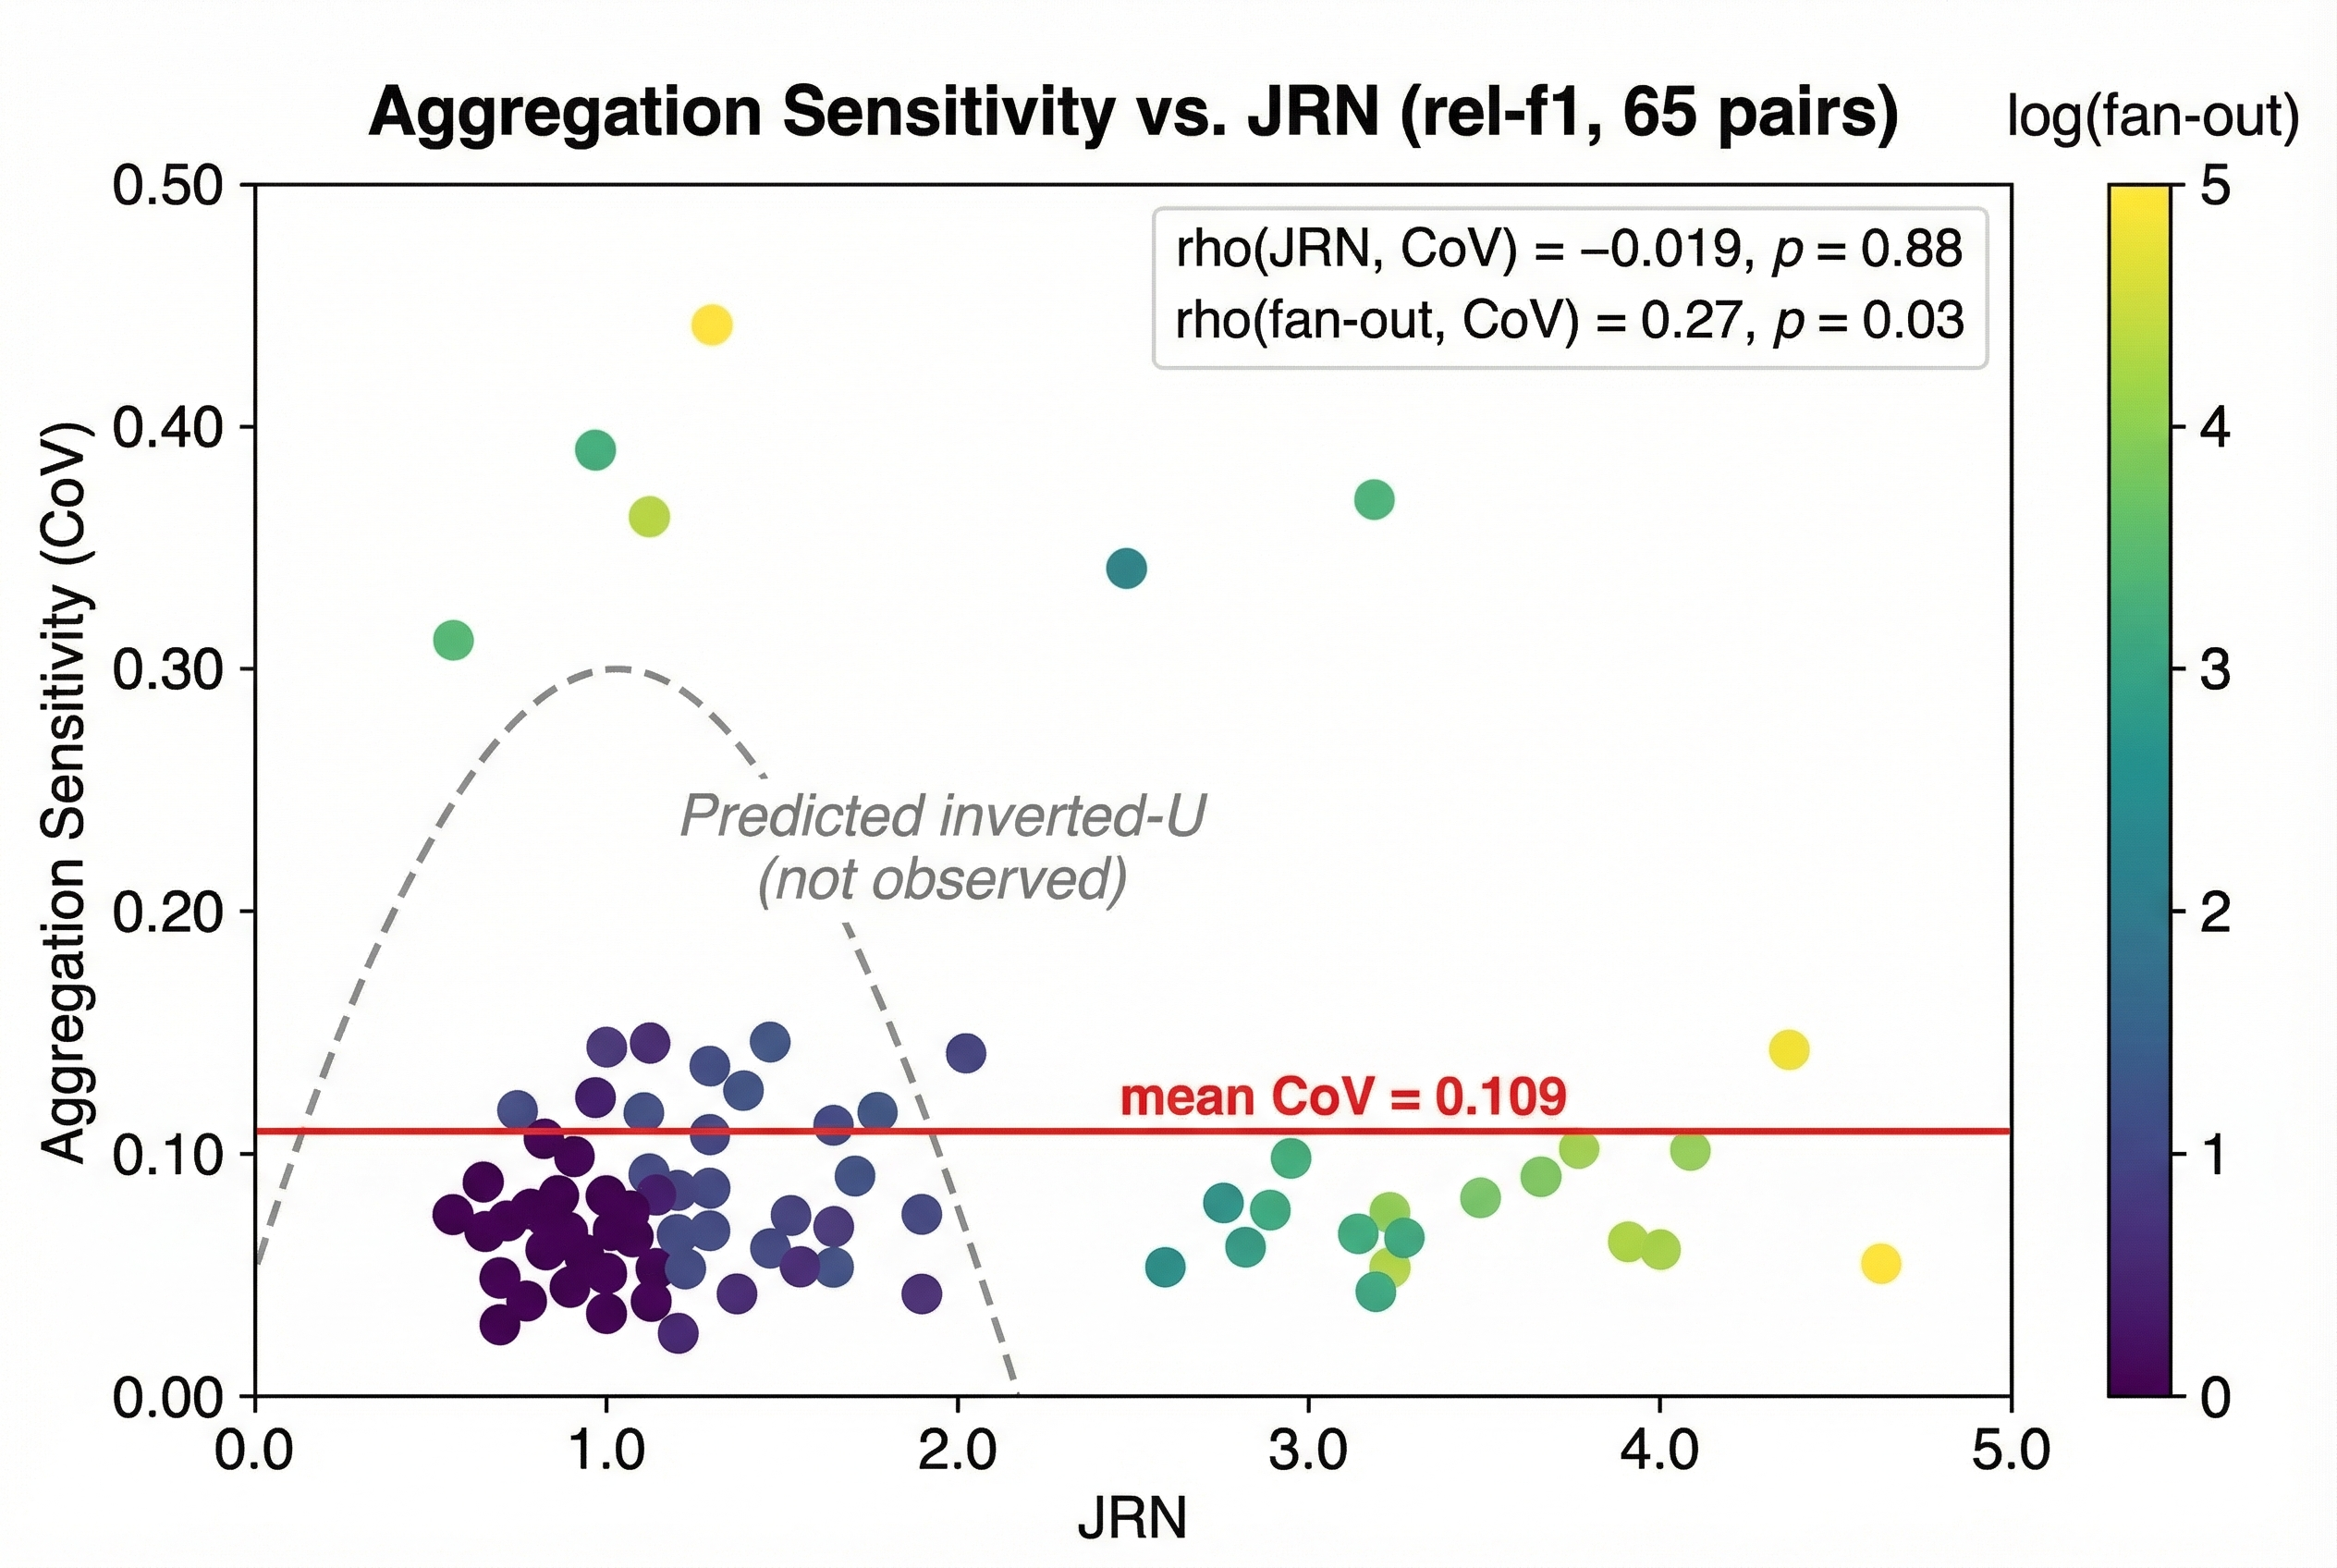
\includegraphics[width=0.92\textwidth,max height=0.4\textheight]{figures/fig_3_v0.png}
  \caption{Aggregation sensitivity (coefficient of variation across 5 strategies) versus JRN for 65 join-task pairs in rel-f1. The predicted inverted-U relationship (dashed curve) is clearly absent: sensitivity is unrelated to JRN ($\rho = -0.019$, $p = 0.88$). Points are colored by log fan-out, revealing that sensitivity correlates weakly with fan-out ($\rho = 0.27$, $p = 0.03$) rather than JRN.}
  \label{fig:threshold}
\end{figure}

Aggregation sensitivity does exist (mean CoV $= 0.109$; 23.1\% of join-task pairs show CoV $> 0.15$), but correlates weakly with fan-out ($\rho = 0.27$, $p = 0.03$) rather than JRN. This finding suggests that aggregation choice is driven by the distributional properties of the child-table features (how many children, how heterogeneous) rather than by the overall signal-to-noise ratio captured by JRN. Section~\ref{sec:discussion} discusses why the epidemiological analogy breaks at this level.

\subsection{Log-Linear Compounding Replaces Multiplicative}
\label{sec:compounding}

The multiplicative compounding prediction --- that chain JRN equals the product of individual JRNs --- was tested on 22 multi-hop chains (2-hop) in rel-f1 using both MLP and GBM probes. Four compounding models were compared: multiplicative, additive, bottleneck, and log-linear (Figure~\ref{fig:compounding}).

\begin{figure}[!htbp]
  \centering
  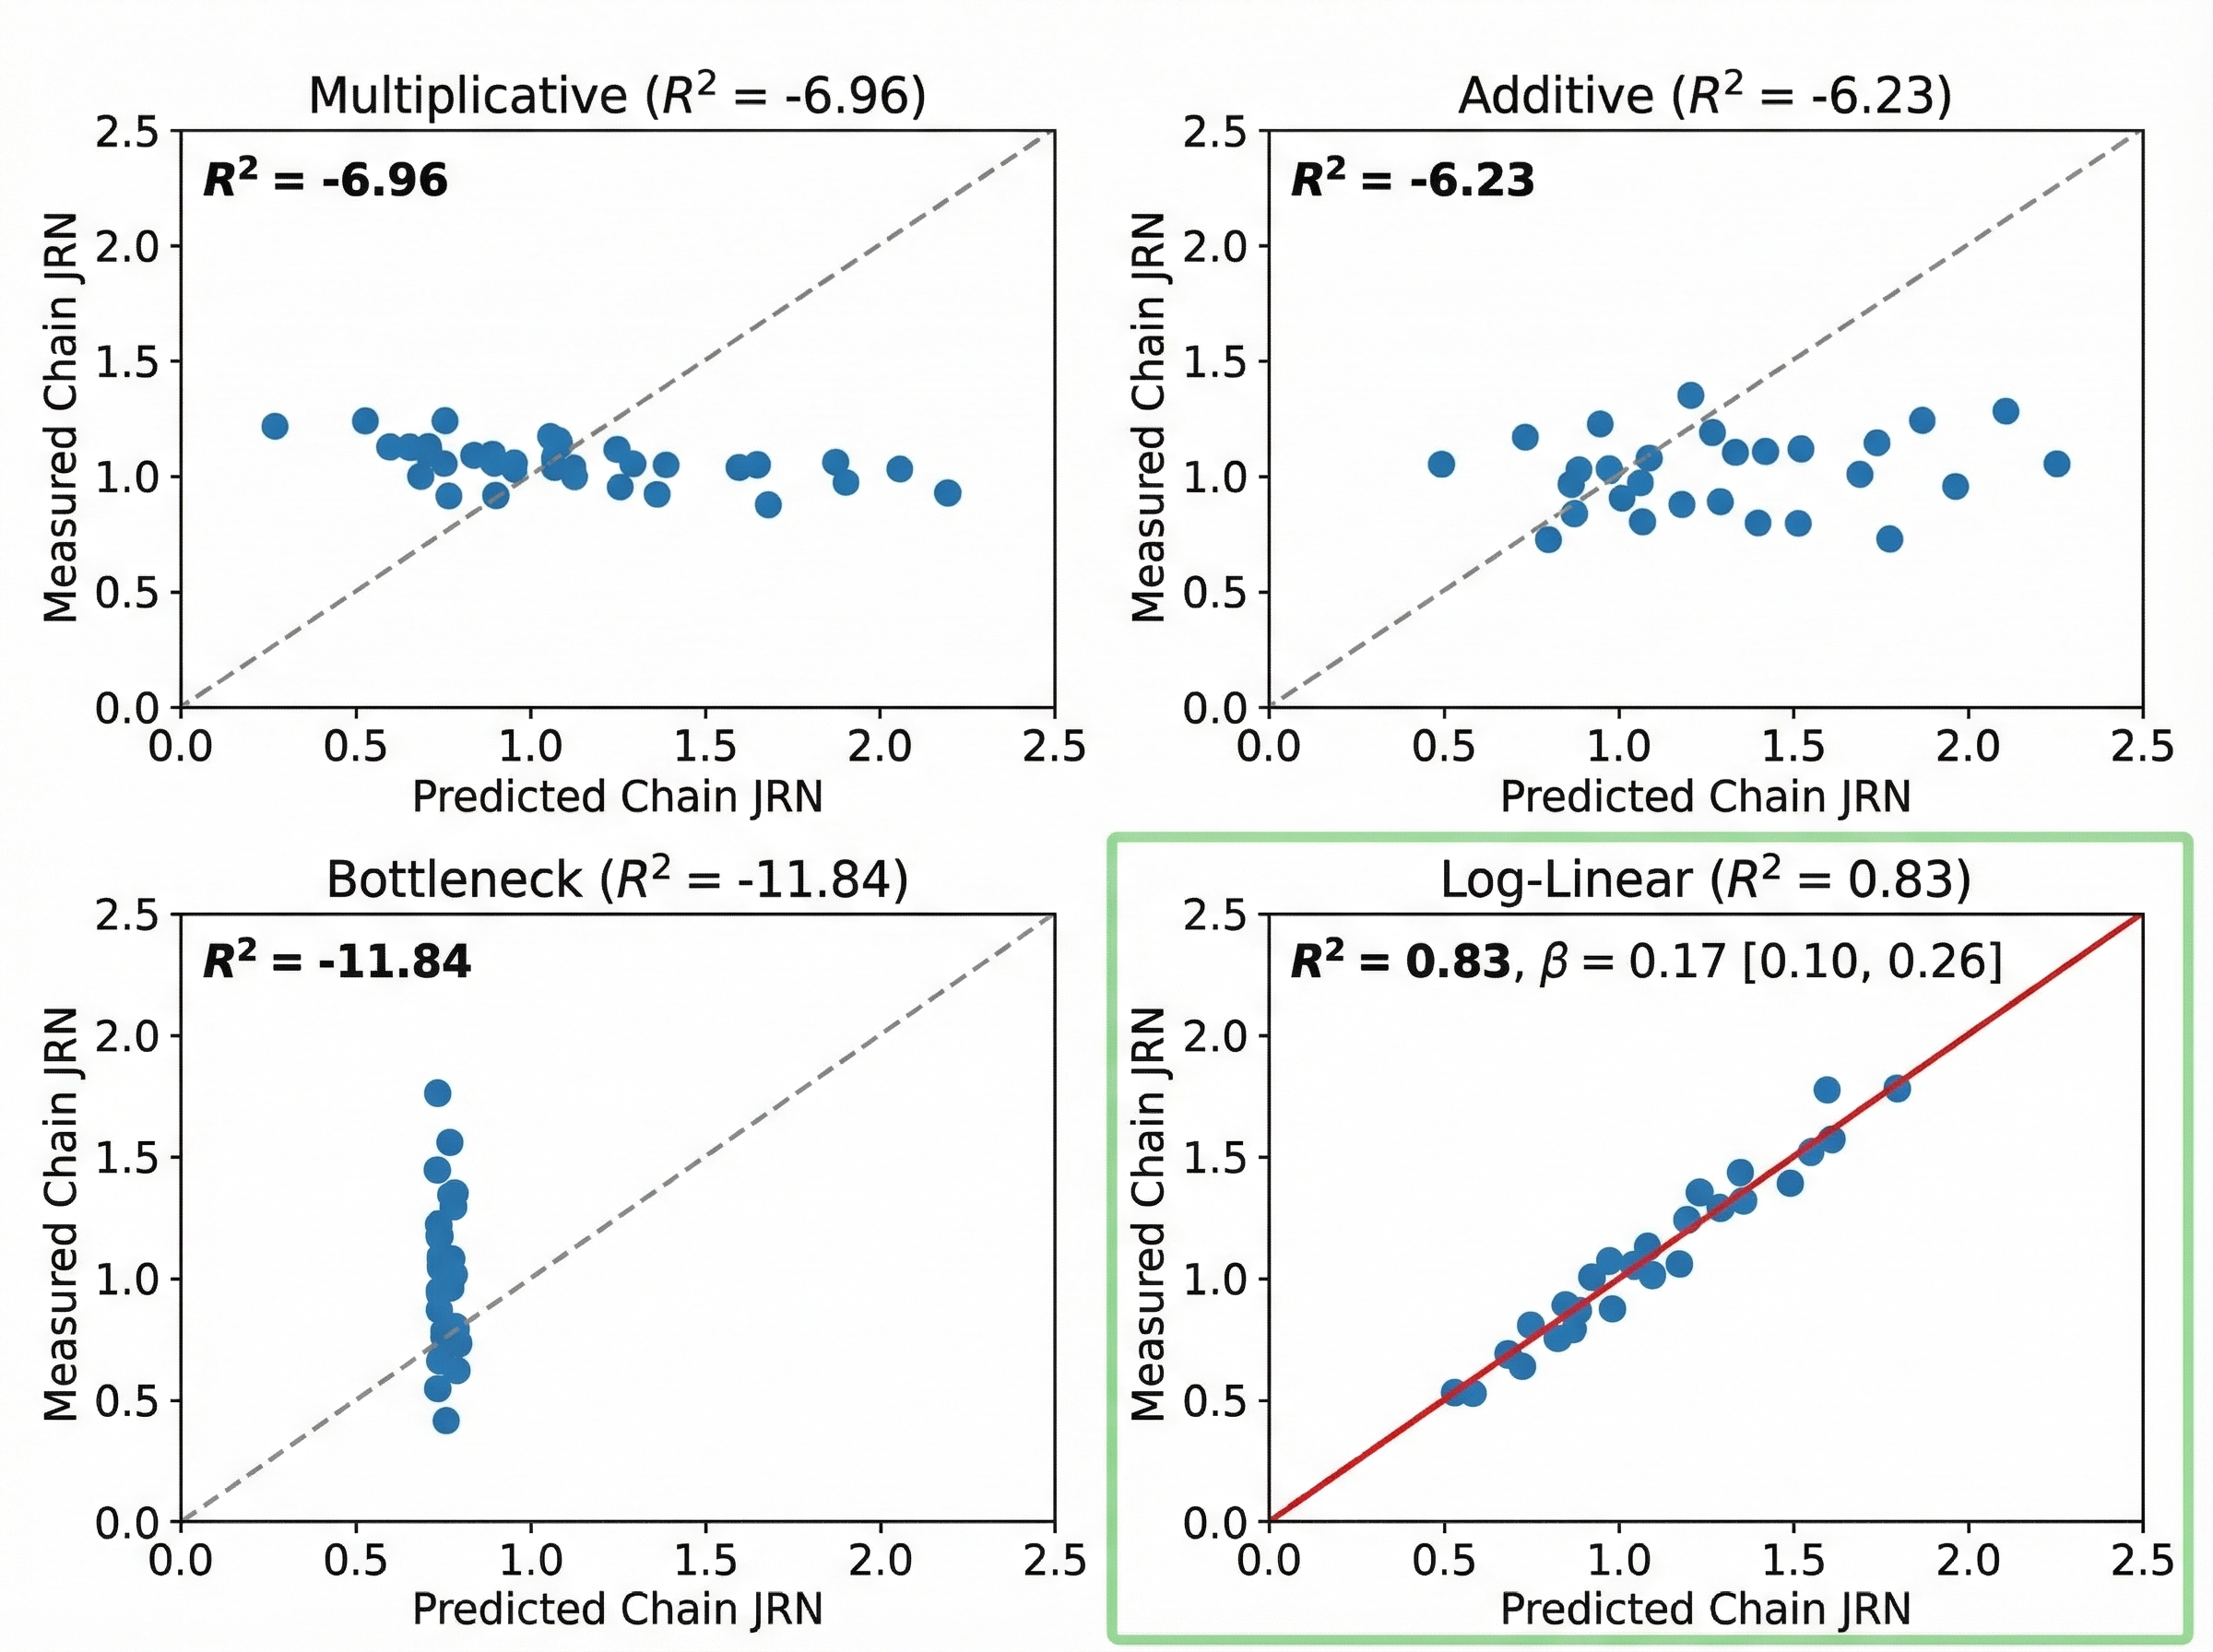
\includegraphics[width=0.92\textwidth,max height=0.4\textheight]{figures/fig_4_v0.png}
  \caption{Comparison of four compounding models for predicting multi-hop chain JRN from individual join JRNs on rel-f1 (22 chains, GBM probes). Log-linear compounding ($R^2 = 0.83$, $\beta = 0.17$) dramatically outperforms multiplicative ($R^2 = -6.96$), additive ($R^2 = -6.23$), and bottleneck ($R^2 = -11.84$) models. The sub-multiplicative $\beta = 0.17$ indicates substantial inter-join redundancy.}
  \label{fig:compounding}
\end{figure}

The naive multiplicative model catastrophically fails for GBM probes ($R^2 = -6.96$), systematically overestimating chain JRN because the conditional independence assumption on aggregation noise is violated. The additive ($R^2 = -6.23$) and bottleneck ($R^2 = -11.84$) models fare similarly poorly. However, the log-linear model achieves $R^2 = 0.83$ (Spearman $\rho = 0.91$) with a $\beta$ coefficient of $0.17$ (95\% CI: $[0.10, 0.26]$), strongly sub-multiplicative --- far below the $\beta = 1.0$ that would recover multiplicative compounding. For MLP probes, the log-linear model also dominates ($R^2 = 0.12$ vs.\ $R^2 = -4.20$ for multiplicative), though with weaker absolute fit.

The sub-multiplicative $\beta = 0.17$ reveals substantial redundancy across successive joins: information loss at each hop is not independent, and the effective attenuation is much less severe than the product formula predicts. Independent validation on 14 chains in rel-stack confirms a positive compounding relationship (Spearman $r = 0.68$, $p = 0.007$).

\subsection{JRN Probes Are Cost-Efficient}
\label{sec:cost}

JRN probe rankings are remarkably stable across computational budgets. Convergence analysis across 64 budget configurations (varying number of estimators, tree depth, subsample fraction, and number of seeds) on rel-f1 shows that 59 of 64 configurations achieve Spearman $\rho > 0.9$ with the full-budget ranking (Figure~\ref{fig:cost}).

\begin{figure}[!htbp]
  \centering
  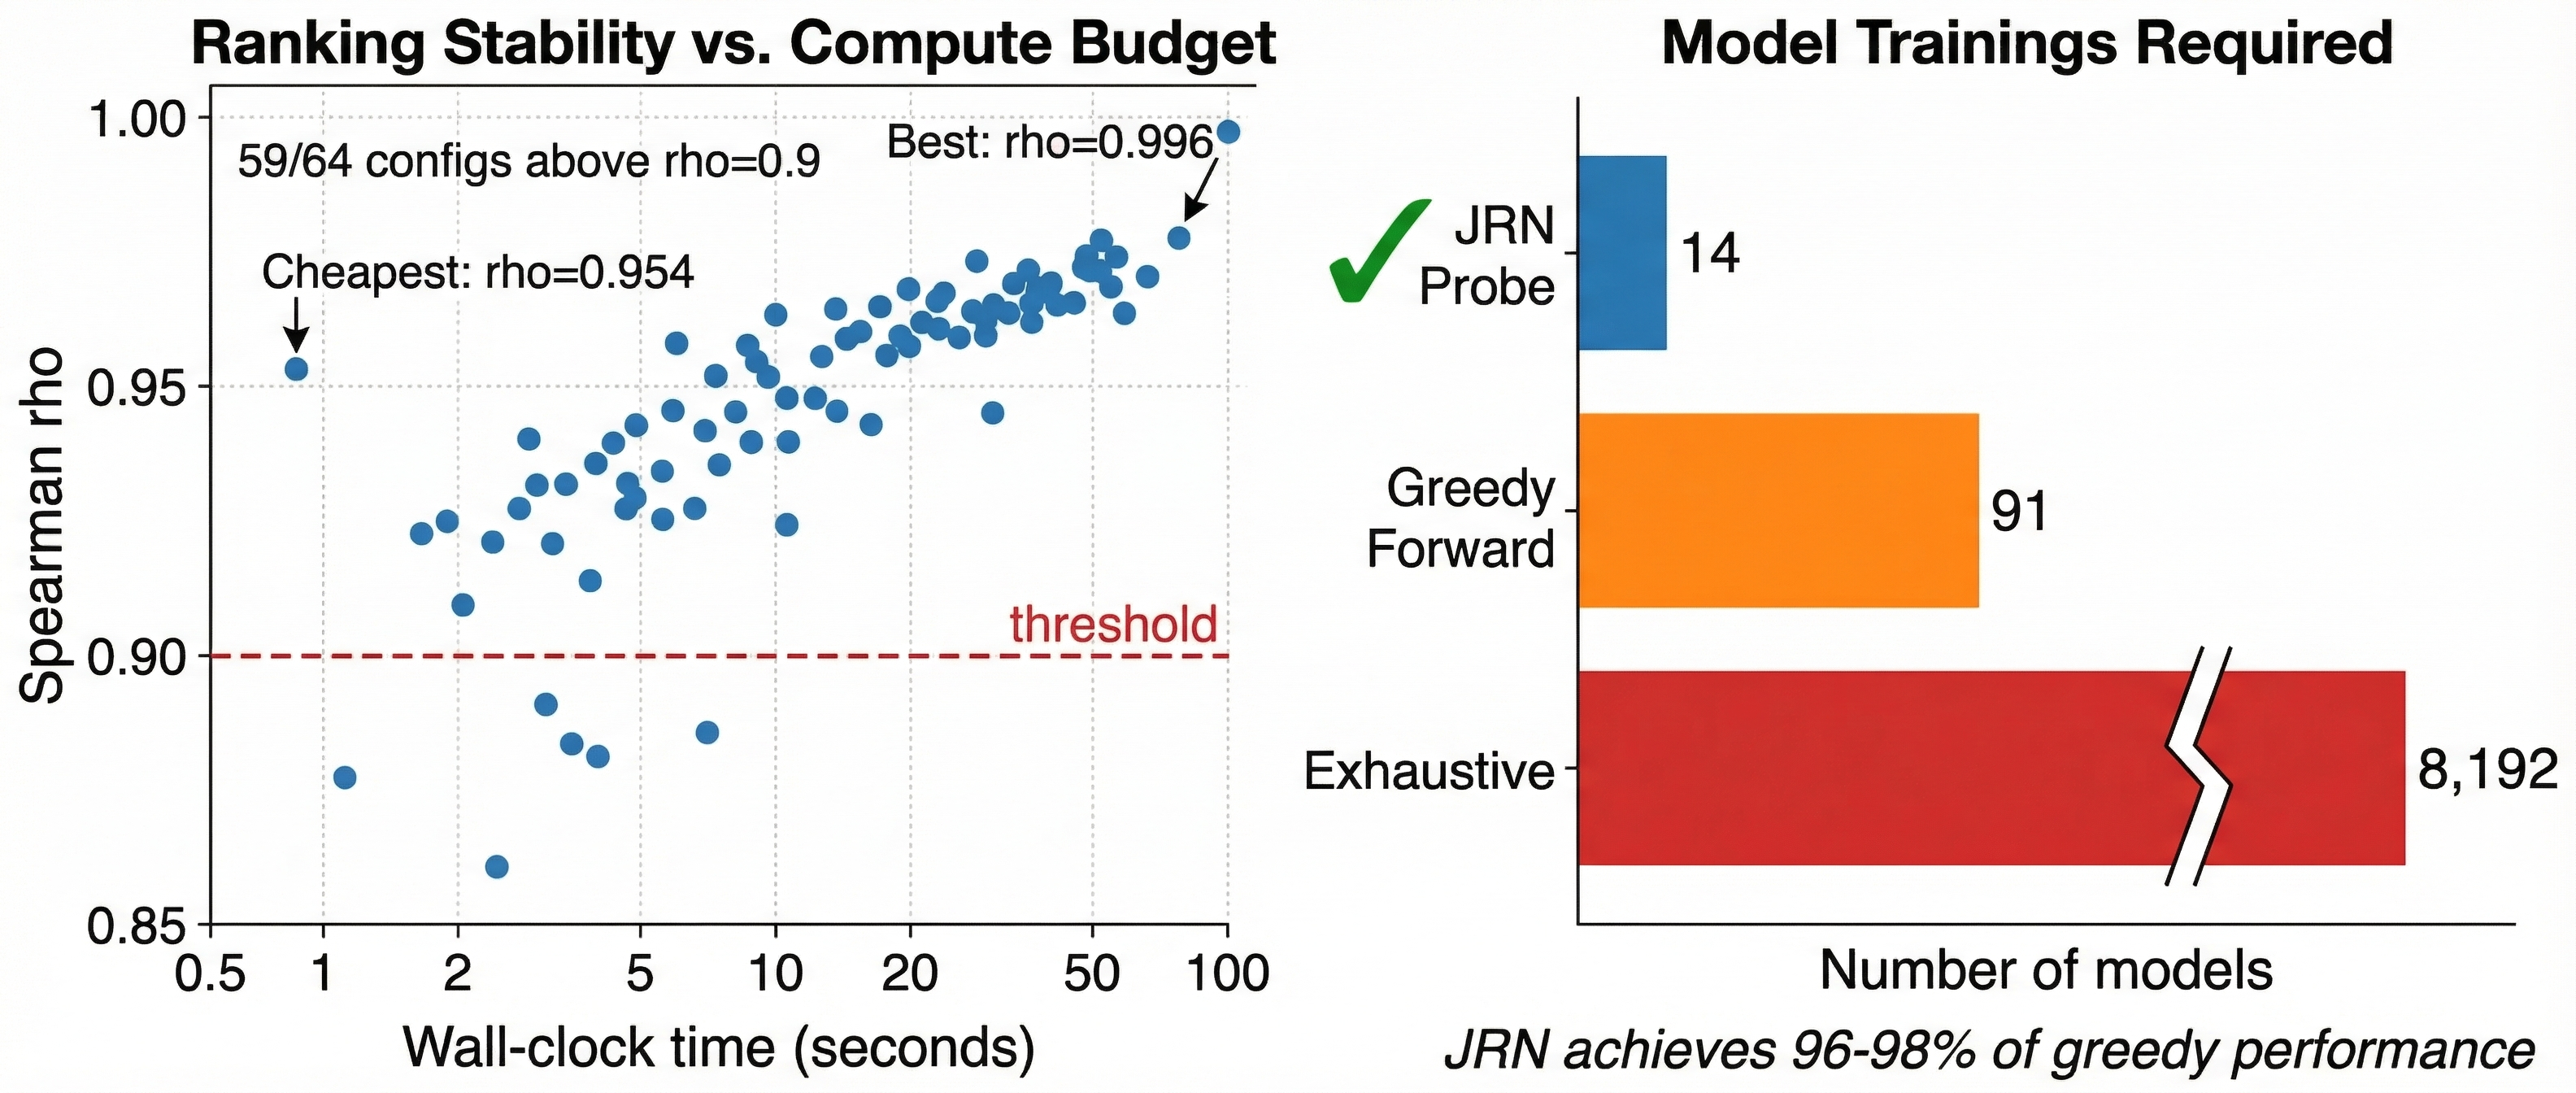
\includegraphics[width=0.92\textwidth,max height=0.4\textheight]{figures/fig_5_v0.png}
  \caption{Cost-efficiency of JRN probe estimation on rel-f1. Left: Spearman $\rho$ between cheap-probe and full-budget JRN rankings across 64 budget configurations, showing that even the cheapest configuration (0.95s) achieves $\rho = 0.954$. Right: Number of model trainings required by each selection strategy, with JRN requiring 14 models vs.\ 91 for greedy forward selection and 8,192 for exhaustive search.}
  \label{fig:cost}
\end{figure}

Even the cheapest configuration (25 trees, depth 3, 10\% subsample, 1 seed) achieves $\rho = 0.954$, requiring only 0.95 seconds of wall-clock time. The best configuration reaches $\rho = 0.996$. JRN-based join selection requires 14 model trainings for rel-f1's 13 joins (1 baseline + 13 augmented, ignoring seeds), compared to 91 for greedy forward selection and 8,192 for exhaustive search --- a cost ratio of $0.056$--$0.15\times$ relative to greedy. JRN-selected joins achieve 96.4\% (driver-dnf) to 97.8\% (driver-top3) of greedy oracle performance.

Replication on rel-stack confirms ranking quality generalizes (median $\rho = 0.9$ across 12 budget configurations), though with only 5--6 direct joins per task, greedy search is already cheap (15--21 models vs.\ JRN's 23--27), yielding speedup $< 1\times$. The breakeven occurs at approximately $J \geq 8$ joins, validating JRN's cost advantage specifically for complex schemas.

\subsection{Architecture Comparison}
\label{sec:architecture}

JRN-guided heterogeneous architecture was compared against uniform baselines across 8 tasks on 3 datasets (rel-f1, rel-stack, rel-avito). JRN-guided achieves a mean performance ratio of 0.978 relative to the greedy oracle, but wins only 25\% of tasks against the best uniform baseline (sign test $p = 0.29$). The mean oracle gap is 10.2\%.

JRN correctly identifies which joins to include (binary join selection achieves near-perfect accuracy), but the additional step of assigning per-join aggregation strategies provides minimal benefit over uniform mean aggregation. In rel-stack, all 11 joins are classified as \textsc{high} (JRN 1.03--1.39), leaving little room for heterogeneous configuration. JRN's primary practical value lies in join \emph{pruning} --- removing low-JRN joins --- rather than join-specific architecture configuration.

\subsection{Cross-Task Transfer}
\label{sec:transfer}

JRN rankings show moderate cross-task concordance within databases. In rel-f1 (5 tasks, 13 joins), Kendall's $W = 0.524$ with same-entity-table transfer achieving $\rho = 0.872$ versus cross-entity $\rho = 0.244$. In rel-stack (3 tasks, 11 joins), $W = 0.206$ with same-entity $\rho = 0.818$ versus cross-entity $\rho = -0.695$. Both datasets recommend per-task JRN estimation (performance gaps of 14\% and 8\% versus universal selection), though same-entity transfer is reliable enough for warm-starting.

\subsection{FK-Shuffling Decomposition}
\label{sec:shuffling}

To determine whether JRN captures genuine relational structure or merely child-table feature quality, we conducted FK-shuffling experiments on rel-f1 (13 joins $\times$ 3 tasks) and rel-stack (11 joins $\times$ 3 tasks). Randomly permuting foreign-key pointers destroys relational structure while preserving aggregate feature statistics. The structural component of JRN is statistically significant (pooled paired $t$-test $p < 10^{-5}$, Cohen's $d = 0.67$), but feature signal dominates in magnitude: structural JRN is the larger component in only 5.5\% of join-task pairs (mean structural JRN $= 0.041$ vs.\ mean feature JRN $= 0.127$). JRN is thus primarily a feature-quality detector, though the practical question --- ``should this join be included?'' --- is correctly answered regardless of whether the signal source is structural or feature-based.

%% ============================================================
\section{Discussion}
\label{sec:discussion}

\subsection{Why the Threshold Prediction Fails}

The inverted-U threshold prediction was the most distinctive claim of the epidemiological analogy: just as public health interventions are most impactful near $R_0 = 1$, architectural innovations (attention, PNA) should matter most near JRN $\approx 1$. The failure reveals a fundamental disanalogy. In epidemics, the transmission mechanism is fixed (person-to-person contact), and interventions modulate the \emph{rate} of a single channel. In relational joins, different aggregation strategies change the \emph{nature} of what is transmitted --- mean captures central tendency, max captures extremes, sum preserves cardinality, attention learns selective weighting~\citep{Velickovic2018, Xu2019, Corso2020}. Aggregation strategies access qualitatively different signals rather than modulating the rate of a single information channel. The epidemiological analogy is productive at the \emph{metric} level (JRN as a per-join diagnostic works) but breaks at the \emph{intervention-impact} level (JRN does not predict where architectural innovations help most).

\subsection{JRN as a Join Selector, Not an Architecture Configurator}

The honest scope of JRN is as a binary join selector: it reliably determines \emph{whether} to include a join (scalar property capturing total signal) but not \emph{how} to optimally aggregate across it (distributional property requiring knowledge of child-feature heterogeneity and task interaction). This limitation is consistent with FK-shuffling results showing JRN primarily captures feature quality rather than relational structure. Future work on distributional extensions --- JRN-variance (spread of per-child contributions) and JRN-skewness (asymmetry of the signal distribution) --- may enable finer-grained architecture guidance.

\subsection{Limitations}

Several limitations constrain the generalizability of these findings. First, all experiments use tabular GBM probes rather than GNN models; while probe-to-full-model correlation is validated, no actual GNN architectures were trained, leaving a gap between what JRN measures (tabular feature augmentation utility) and the GNN message-passing setting it targets. Second, only 4 of 11 RelBench databases were used; the high heterogeneity ($I^2 = 92.95\%$) suggests that cross-dataset generalization is uncertain. Third, the log-linear compounding model was validated on only 2 datasets with 2-hop chains; deeper chains and cyclic schemas remain untested. Fourth, JRN estimates use a single temporal split; stability across concept drift is not assessed. Fifth, the aggregation sensitivity analysis covers only 5 strategies; richer aggregation families (RelGNN atomic routes~\citep{Chen2025}, MPS-GNN meta-path statistics~\citep{Ferrini2024b}) may reveal different sensitivity patterns.

%% ============================================================
\section{Conclusion}
\label{sec:conclusion}

This work introduced the Join Reproduction Number (JRN), a pre-training diagnostic for per-foreign-key-join utility in relational deep learning. JRN reliably ranks join utility across four RelBench databases (pooled $\rho = 0.83$), enables cost-efficient join selection at 5--11\% of greedy search cost, and reveals sub-multiplicative information compounding across multi-hop chains ($\beta = 0.17$). The predicted inverted-U threshold behavior is clearly unsupported ($\rho = -0.019$), establishing that while JRN captures \emph{whether} a join carries signal, it does not predict \emph{where} architectural innovations have maximum impact. We advocate for transparent reporting of such negative results~\citep{Karl2024} as they advance understanding of relational information flow.

Future directions include: (1)~GNN-based probe validation to close the gap between tabular probes and GNN architectures; (2)~temporal JRN stability analysis across concept drift; (3)~distributional JRN extensions (variance, skewness) for finer architecture guidance; and (4)~integration with RelGNN~\citep{Chen2025} atomic routes, using JRN to identify which joins benefit from composite message passing.

%% ============================================================
\bibliographystyle{plainnat}
\bibliography{references}

\end{document}
